\documentclass[12pt]{article}
\usepackage[margin=0.9in]{geometry} 
\usepackage{amsmath}
\usepackage{tcolorbox}
\usepackage{hyperref}
\usepackage{amssymb}
\usepackage{amsthm}
\usepackage{graphicx}
\usepackage{lastpage}
\graphicspath{ {./} }
\usepackage{fancyhdr}
\usepackage{accents}
\pagestyle{fancy}
\setlength{\headheight}{40pt}


\newenvironment{solution}
  {\renewcommand\qedsymbol{$\blacksquare$}
  \begin{proof}[Solution]}
  {\end{proof}}
\renewcommand\qedsymbol{$\blacksquare$}

\newcommand{\ubar}[1]{\underaccent{\bar}{#1}} % add packages, settings, and declarations in settings.tex


\begin{document}

\lhead{Crețu Cristian} 
\rhead{clasa a XI-a} 
\cfoot{\thepage\ din \pageref{LastPage}}


\textbf{\LARGE Protecția persoanelor și a mediului împotriva efectelor nocive ale sunetului și reducerea zgomotului
}

\vspace{0.5cm}
Poluarea fonică reprezintă o problemă din ce în ce mai mare în întreaga lume și este posibil ca mulți oameni să nu realizeze efectul ei asupra sănătății.

\section{Elemente de acustică}

\quad Urechea umană percepe vibrațiile care au frecvența cuprinsă între 16 și 20.000 Hz. Vibrațiile sub 16 Hz se numesc infrasunete (generate de cutremure, stații de amplificare, etc) și cele peste 20.000 Hz se numesc ultrasunete. După senzațiile produse asupra urechii, sunetele se clasifică în \textbf{detonații} - (sunete cu durata foarte scurtă și intensitate mare) și \textbf{zgomote} - (în general, vibrații mecanice aperiodice).\footnote{Cleopatra \& Nicolae Gherbanovschi - Manualul de fizică pentru clasa a XI-a, pag.37}

Caracteristicile fizice sau obiective ale zgomotului privesc tăria sau intensitatea sonoră, durata și frecvența. Intensitatea este caracterul cel mai important care depinde de trăsăturile sursei, de distanță și posibilitățile de transmitere sau multiplicare. Ea se măsoară în decibeli sau foni. ${\displaystyle X_{dB}=10\log _{10}(X)}$ (un decibel este a 10-a parte dintr-un Bel).

\section{Poluare acustică}

\quad Atunci când estimăm riscul de deteriorare a auzului trebuie luați în calcul trei factori importanți: timpul de expunere, frecvența (Hz) și presiunea acustică (dB). Timpul de expunere este măsurat pe o perioadă de 8 ore, pentru a simula un mediu de lucru standard. Este utilizat un filtru (dB A), care ține cont de curba de toleranță normală a urechii umane și asigură o estimare corectă a nivelului de risc.\footnote{\href{https://ro.wikipedia.org/wiki/Decibel}{Wikipedia - Decibel}}

Zgomotele de frecvență înaltă sunt cele mai nocive pentru auz și, ca urmare, reprezintă principalul motiv de îngrijorare.

Zgomotele de frecvență joasă sunt de obicei mai puțin nocive, dar pot fi periculoase deoarece acoperă vocea umană, semnalele de alarmă și poate cauza stări de amețeală sau de greață.

Pierderea auzului de înaltă frecvență este frecventă și tinde să progreseze odată cu vârsta. \href{https://web.archive.org/web/20201107234502if_/https://www.humanbenchmark.com/tests/hearing}{Human Benchmark} - este un test care determina cea mai mare frecvență auzibilă.

Potrivit unui studiu publicat de Organizația Mondială a Sănătății, poluarea acustică produsă de trafic stă la originea unor boli, disfuncții și morți premature. Zgomotul produs de mijloacele de transport poate provoca diverse tulburări, de la insomnie la infarct, probleme de învățare, acufene (țiuituri în urechi) spasme stomacale, tresărirea și reținerea respirației, tensionarea musculaturii, dilatarea pupilelor sau chiar moartea. Potrivit studiului, zgomotul provocat de traficul rutier este al doilea factor de mediu favorizant al îmbolnăvirilor, după poluarea atmosferică. În anul 2015, se estima că aproximativ 10.000 de persoane mor anual, în întreaga lume, din cauza afecțiunilor asociate poluării sonore din marile orașe.

Pragul inferior, dedesubtul căruia sunetele nu mai sunt sesizate de urechea umană este însemnat prin 0 decibeli. Limita superioară este de aproximativ 140 de decibeli, dincolo de care sunetele nu mai pot fi auzite corect, deoarece intensitatea prea mare distorsionează perceperea auditivă, producând chiar senzații dureroase. Supradimensionarea intensității unor sunete sau zgomote peste limitele fiziologice admise sau expunerea pe timp îndelungat la poluare fonică, au drept consecință deteriorarea și compromiterea aparatului auditiv.\footnote{\href{https://ro.wikipedia.org/wiki/Intensitate_sonoră}{Wikipedia - Intensitate sonoră}}

\begin{figure}[h]
    \centering
    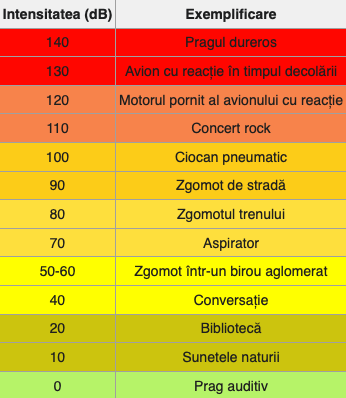
\includegraphics[width=0.4\textwidth]{db_table}
    \caption{Tabelul intesităților sunteului}
    \label{fig:mesh1}
\end{figure}

\section{Măsuri de prevenire}

\quad Țările, regiunile și
 orașele iau numeroase măsuri pentru a soluționa problemele legate de zgomot. De exemplu, folosirea de asfalt fonoabsorbant pe drumurile publice, utilizarea de anvelope silențioase la vehiculele de transport public, dezvoltarea infrastructurii pentru automobile electrice în orașe, promovarea mobilității active, cum ar fi mersul pe jos sau cu bicicleta, transformarea străzilor în zone pietonale etc. De asemenea, un număr semnificativ de orașe și regiuni au introdus așa-numite zone liniștite, unde oamenii pot evada din zgomotul orașului. Acestea sunt în mare parte spații verzi, cum ar fi parcuri sau rezervații naturale.\footnote{\href{https://www.eea.europa.eu/ro/articles/poluarea-fonica-este-o-problema}{Agenția Europeană de Mediu}}

Un pericol proeminent este expunerea unor intensități ridicate la căști. Telefoanele noi conțin o măsura bună pentru prevenirea poluarii fonice: headphone safety atât monitorizează expunerea la sunete cu o intensitate mare cât și avertizează utilizatorul de pericol. Exista și o facilitate de a limita volumul la o anumită intensitate, reducând audioul peste acea limită.

În plus, Uniunea Europeana produce constant noi directive și norme precum \href{https://eur-lex.europa.eu/legal-content/RO/TXT/?uri=CELEX:32014R0598}{normele UE privind zgomotul produs de aviație} sau \href{https://eur-lex.europa.eu/legal-content/RO/ALL/?uri=CELEX:32002L0049}{Directiva-cadru privind zgomotul ambiental} ce urmăresc reducerea expunerii la zgomotul ambiental prin armonizarea indicatorilor de zgomot și a metodelor de evaluare a acestuia.

\end{document}
